\documentclass[oneside]{article}
\usepackage[a4paper]{geometry}
\geometry{verbose,tmargin=3.5cm,bmargin=3cm,lmargin=3cm,rmargin=3cm}

\usepackage{graphicx}
\usepackage{lmodern}
\usepackage[T1]{fontenc}
\usepackage[utf8]{inputenc}

\usepackage{url}
\usepackage{multirow}
\usepackage[unicode=true, bookmarks=true, bookmarksnumbered=true, bookmarksopen=false, breaklinks=false, pdfborder={0 0 0}, pdfpagemode=UseNone, backref=false, colorlinks=true]{hyperref}
\hypersetup{
    colorlinks=true,
    linkcolor=black,
    filecolor=magenta,
    urlcolor=cyan,
    pdftitle={Road crossing cost algorithm},
    pdfstartview=,
}
\urlstyle{same}

\usepackage{mathtools}
\usepackage{mathbbol}
\usepackage[italicdiff]{physics}
\usepackage{float}
\usepackage{pgfplots}
\usepackage{tikz}
\pgfplotsset{compat=1.16}
\usepgfplotslibrary{polar}

\usepackage{fancyhdr}
\pagestyle{fancy}
\fancyhf{}
\setlength{\headheight}{27.51pt}
\usepackage{titling}
\fancyhf[HC]{\LARGE \thetitle}
\fancyhf[HR]{\theauthor}
\fancyhf[HL]{
\includegraphics[height=20pt]{electrical_engeneering_cb.pdf}}
\fancyhf[FR]{\thepage}

\title{Road crossing cost algorithm}
\author{CTU VRAS}
\date{\today}

\begin{document}
    \section{Algorithm overview}
    This algorithm was designed to evaluate and set costs for individual road segments based on their suitability for crossing. It consists of multiple steps. First one is identifying roads in osm data\footnote{Open street map data downloaded with Overpass API.} of the target area. Second is calculating intermediate cost functions based on different parameters. One evaluates curves and distances from them as well as distances from road junctions, other evaluates terrain irregularities and their effect on visibility, and the last evaluates the suitability for crossing based on road classification. Last step combines the previous three cost functions into final crossing cost, and passes this information to our pathfinding algorithm.

        \subsection{Road identification}
        Identifying road segments is relatively easy as all road segments have a "highway" tag and generaly speaking are ways. We therefore select all ways that match this description and convert them into LineString objects.
        
        Once we have our road network created, we detect all intersecting points of individual LineString road objects. From these intersection we later select all points that mark junctions, junctions are intersection points where there are at least three roads connecting. To these points we add all points representing T-shaped junctions, which we detect as road end points connecting with a non end point of another road.

        \subsection{Road curvature}
        \label{sec:rd_cur}
        The idea behind this part of the cost function is that near junctions and curves we cannot see incoming vehicles very clearly. Making road segments near these features less suitable for crossing than lets say segments of a long straight road.

        We already have the positions of all junctions in our road network from previous step.

        The evaluation of the road curvature is based on radii of circumcircles of triangles made from points on road in which the road change direction. Equation (\ref{eqn:circum_circle}) shows how to calculate the circumcircle radius. Figure \ref{fig:curvature} shows why the circumcircle radius is being used to determine road curvature.

        \begin{equation}
            r = \frac{(a\cdot b\cdot c)}{\sqrt{(a+b+c)\cdot(a+b-c)\cdot(a+c-b)\cdot(b+c-a)}},
            \label{eqn:circum_circle}
        \end{equation}

        \noindent where a,b,c are the lengths of respective triangle sides. As we know the precise coordinates of all three vertices, we are able to calculate all neccessary values to later evaluate the radius. 

        We have 6 levels of "curvature". The highest level is reserved for segments near junctions, other segments curvature levels are determined from their circumcircle radius. The curvature value is then set by the segments length multiplied by the segments curvature level weight.
        
        The final value of segments cost is then calculated in following manner. We take a segment and look in both directions of travel from the segment. We go in one of the directions and sum the values of segments curvature we encounter until we get to an exploratory range limit or we reach the end of the road, then we do the same in the other direction. In the end we divide the sum by the length of the explored road, floor the value and set it as the final cost of curvature for this segment.

        \begin{figure}[H]
            \centering
            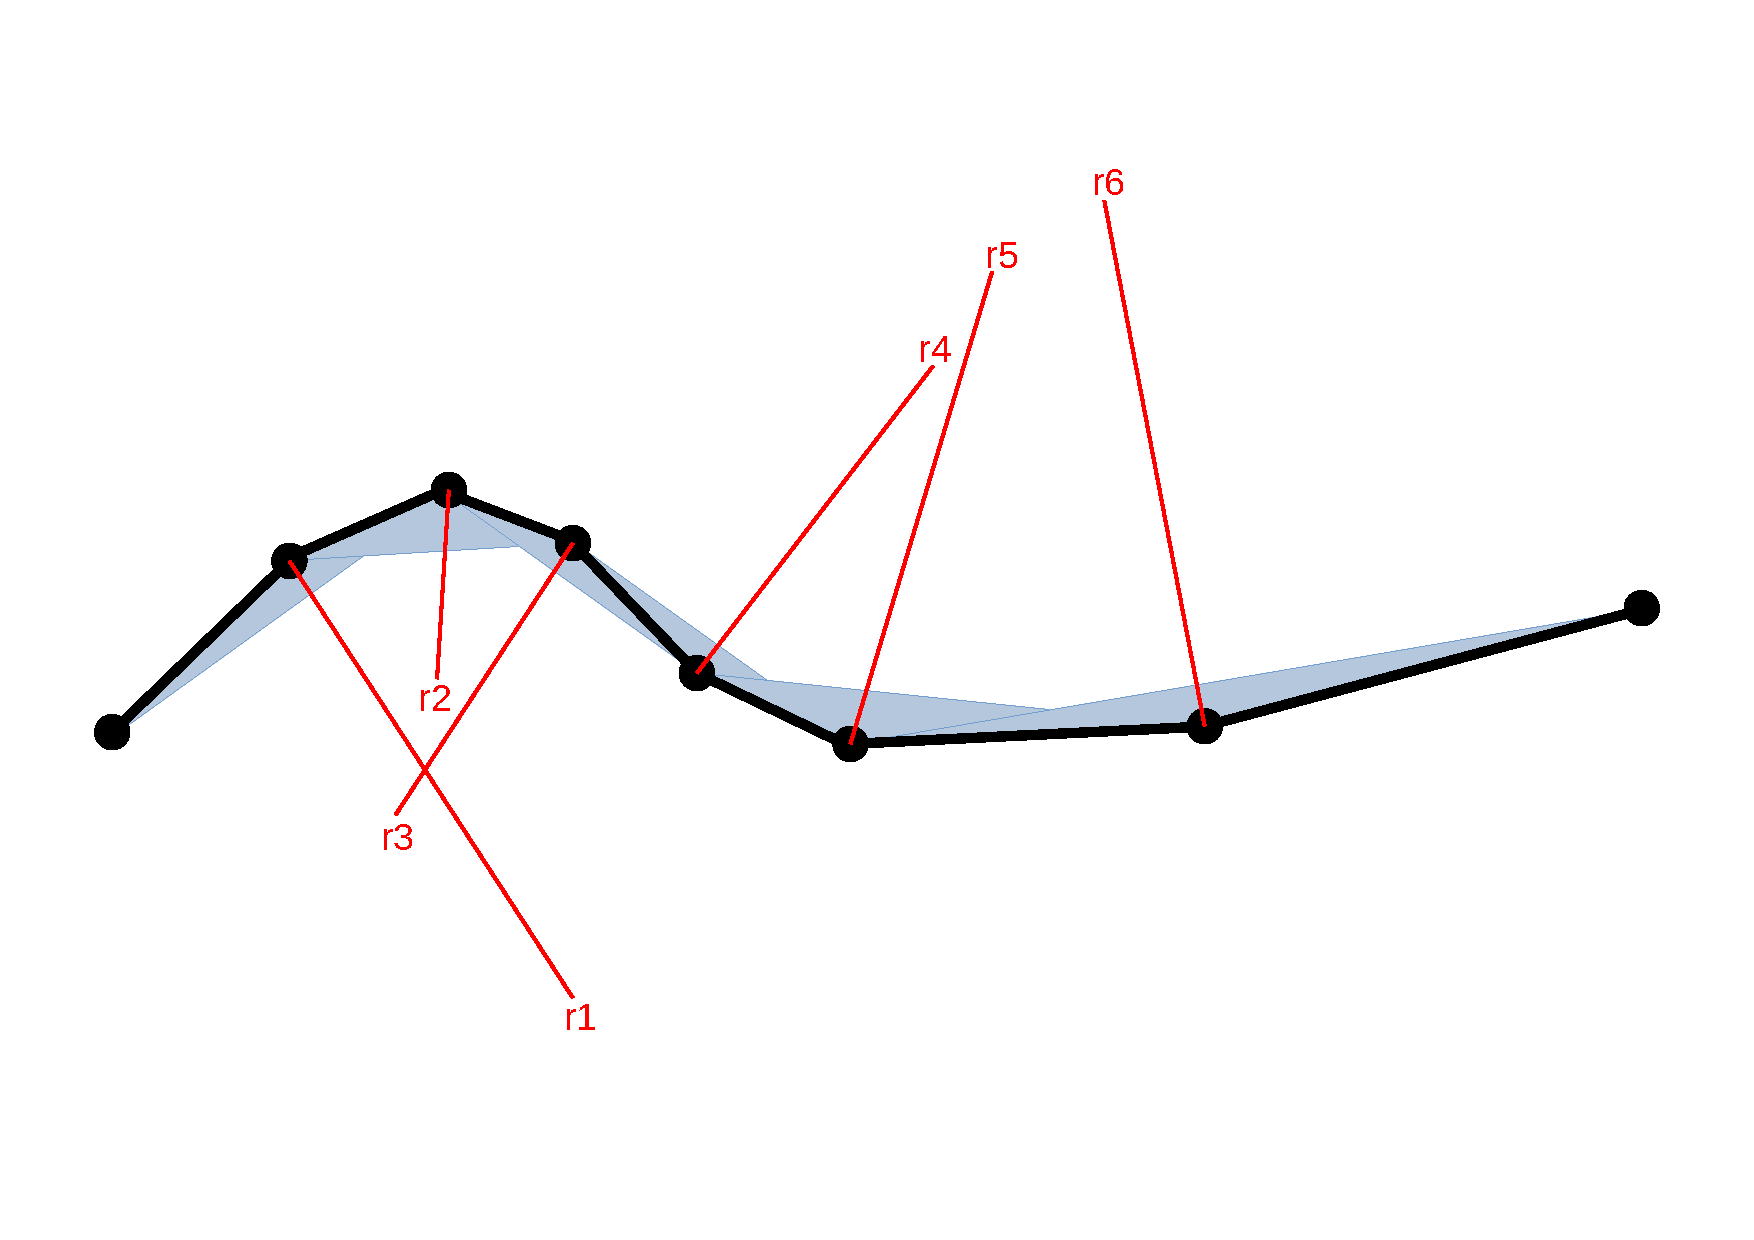
\includegraphics[trim={0cm 3.5cm 0cm 2.7cm}, clip, width=\linewidth]{path_curvature.pdf}
            \caption{Visualization of circumcircles radii in road curvature evaluation.}
            \label{fig:curvature}
        \end{figure}

        \subsection{Road elevation}
        The idea behind this part is based on reduced visibility near terrain irregularities. 

        We take the road network that we have prepared in first step and divide each road into equidistant segments. We than assign height to the dividing points, the height assignment takes five nearest points from the elevation data\footnote{We use data from the Czech Land Survey Office -- ZABAGED\textsuperscript{\textregistered}\ 5G.}, and calculates the height in following manner

        \begin{equation}
            e=\sum_{i=1}^{5}e_{i}\cdot\frac{\sum_{j=1}^{5}d_{j}}{d_{i}},
        \end{equation}

        \noindent where $e_{i}$ is elevation of the i-closest points and $d_{i}$ is the distance of these points from our desired point.

        After we have heights assignt to road points we classify each point with TPI landform classification. We use a modified version of the classification that uses two intervals (smaller and larger one). The main difference is that instead of two-dimensional interval we only use one-dimensional interval, and the limiting constants are slightly altered. The equation (\ref{egn:TPI}) shows how we calculate the value we later evaluate.

        \begin{equation}
            TPI=e_{0}-\frac{\sum_{i=1}^{N}e_{i}}{N},
            \label{egn:TPI}
        \end{equation}

        \noindent where $e_{0}$ is elevation of the point of evaluation, $e_{i}$ is elevation of points within boudaries, $N$ is the number of total points in the evaluation.

        For all points we have two values, one for smaller and one for larger boundary. Based on these two values and limiting constants we can classify each point as one of ten different classes. Five of them are shown in figure \ref{fig:TPI}.

        \noindent The classes are:
        \begin{itemize}
            \item Canyons -- SN: TPI $\le$ $-$s\_limit, LN: TPI $\le$ $-$l\_limit
            \item Midslope drainages -- SN: TPI $\le$ $-$s\_limit, LN: $-$l\_limit $<$ TPI $<$ l\_limit
            \item Upland drainages -- SN: TPI $\le$ $-$s\_limit, LN: TPI $\ge$ l\_limit
            \item U-shaped valleys -- SN: $-$s\_limit $<$ TPI $<$ s\_limit, LN: TPI $\le$ l\_limit
            \item Plains -- SN: $-$s\_limit $<$ TPI $<$ s\_limit, LN: $-$l\_limit $<$ TPI $<$ l\_limit, slope $\le5^{\circ}$
            \item Open slopes -- SN: $-$s\_limit $<$ TPI $<$ s\_limit, LN: $-$l\_limit $<$ TPI $<$ l\_limit, slope $>5^{\circ}$
            \item Upper slopes -- SN: $-$s\_limit $<$ TPI $<$ s\_limit, LN: TPI $\ge$ l\_limit
            \item Local ridges -- SN: TPI $\ge$ s\_limit, LN: TPI $\le$ $-$l\_limit
            \item Midslope ridges -- SN: TPI $\ge$ s\_limit, LN: $-$l\_limit $<$ TPI $<$ l\_limit
            \item Mountain tops -- SN: TPI $\ge$ s\_limit, LN: TPI $\ge$ l\_limit
        \end{itemize}

        We have a cost associated with each of these classes, and the final cost of the segments is evaluated in the same way as final evaluation for road curvature with only one change, here we do not count the cost of the segment we are evaluating.

        \begin{figure}[H]
            \centering
            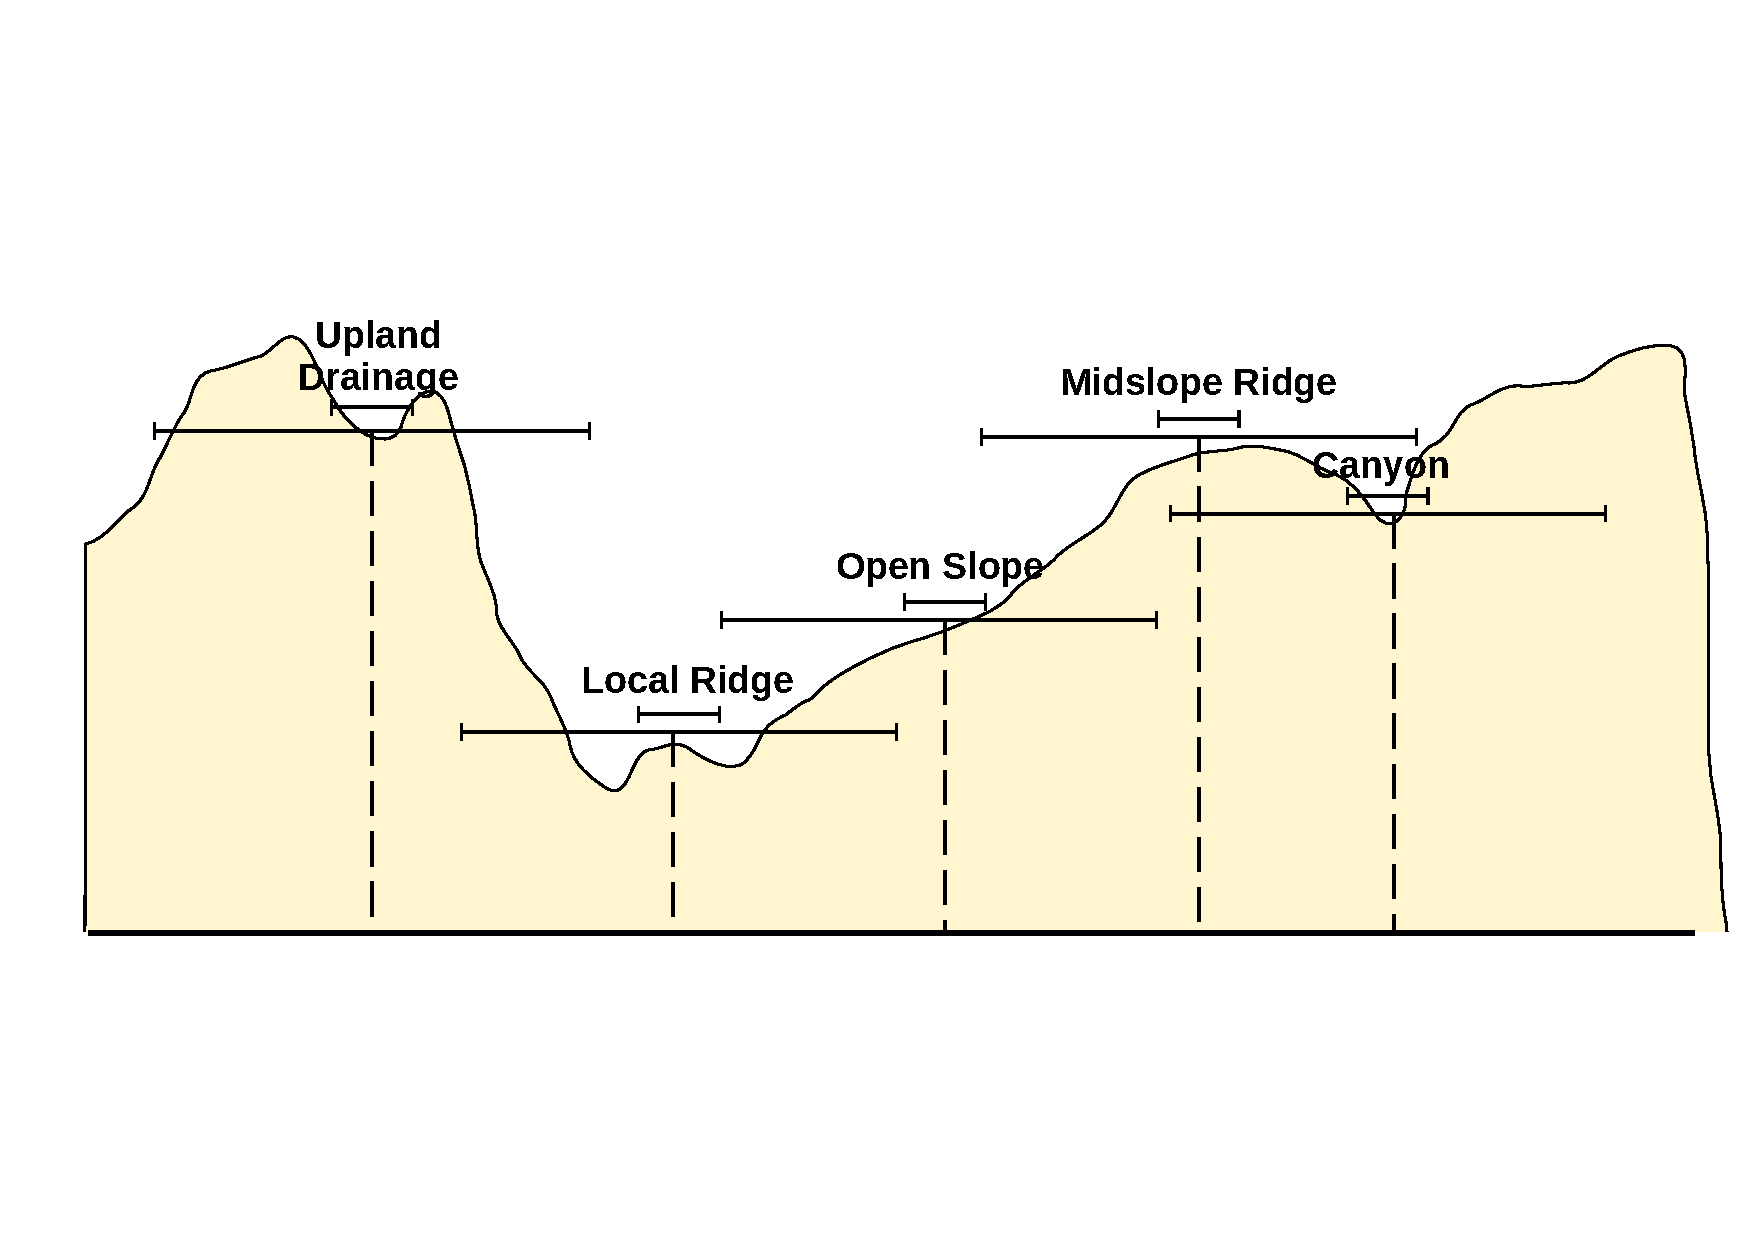
\includegraphics[trim={1.5cm 5.2cm 1.2cm 5.4cm}, clip, width=\linewidth]{TPI_classification.pdf}
            \caption{Visualization of a few TPI landform classes.}
            \label{fig:TPI}
        \end{figure}

        \subsection*{Road classification}
        The idea behind this part of cost algorithm is that lower tier roads are more suitable for crossing than higer tier ones. Generally speaking on lower tier roads cars are driving more slowly and less frequently. The osm provides multitude of different highway classifications some of we identify as footways and do not consider them a road that needs to be crossed carefuly.

        \noindent The following road classification are the ones we evaluate, roads on the same line have same cost associated with them:
        \begin{itemize}
            \item Primary, primary link
            \item Secondary, secondary link
            \item Tertiary, tertiary link
            \item Residential, living street
            \item Busway
            \item Unclassified
            \item Road
            \item Service
        \end{itemize}

        \subsection{Algorithm constants}
        We can easily modify the function of the algorithm by tweaking the following constants, that our found in a file road\_crossing\_consts.py:
        \begin{itemize}
            \item Weights for the 6 levels of road curvature
            \item Maximal radius for each level of road curvature
            \item Cost for individual road classifications
            \item Number of levels in individual parts of road crossing cost algorithm (curvature, elevation, classification, final)
            \item Weights of intermediate cost functions relative to final cost
            \item Number of points in batch in elevation assignment (impacts speed)
            \item Interval and limiting constants in TPI landform classification
            \item Costs for individual types of TPI landform classes
        \end{itemize}

    \newpage
    \section{Algorithm implementation}
    The whole algorithm is divided into several files for easier manipulation.

    \noindent The files in which the algorithm is divided are:
    \begin{itemize}
        \item road\_detection.py
        \item road\_curvature.py
        \item road\_elevation.py
        \item road\_crossing\_consts.py
    \end{itemize}

        \subsection{road\_detection.py}
        In this file there are methods used to create road network, find intersections and junctions and overall prepare osm data for further work.

            \subsubsection{get\_roads(data)}
            This method returns list of all roads we consider crossable, meaning they have one of the following higway tags: primary, primary\_link, secondary, secondary\_link, tertiary, tertiary\_link, unclassified, residential, service, busway, road, living\_street.

            The input data is the osm data query we get from Overpass API of the target area.

            The return value is a list of tuples, each tuple represents one road in the osm data. First value of the tuple is list of tuples, these tuples represent nodes the road is made of, first value of the tuple is the nodes id, second value is the nodes lattitude and third value is the nodes longitude. Second value of the road tuple is the roads classification.

            \subsubsection{gps\_to\_utm(data, withID)}
            This method returns a numpy array of gps lattitude and longitude coords transformed into UTM format.

            The input data is a list of tuples with coords in gps lat and lon to be transformed into UTM.

            The input withID is a bool value that specifies if the tuples in input data list have an ID in the first position. The default value is true.

            The return value is a numpy array where the lat and lon values have been transformed into utm format.

            \textbf{Example:}\\
            \noindent input: data = [()], withID = false\\
            \noindent output: [[]]

            \subsubsection{create\_line\_for\_road(road, withID)}
            This method creates shapely.geometry.LineString object for road nodes.

            The input road is a list of tuples with coords in UTM format.

            The input withID is a bool value that specifies if the tuples in input data list have an ID in the first position. The default value is true.

            The return value is a LineString object that has been created from the road nodes coordinates.

            \subsubsection{create\_road\_network(roads, inUTM, withID)}
            This method creates shapely.geometry.MultiLineString object for all roads in the osm data of target area. We firstly create a LineString object for individual roads and then combine them into one MultiLineString object. This object is the road network structure we use in further parts of the algorithm.

            The input roads is a list of lists of tuples. The each list inside this list represents one road for which we create a LineString object.

            The input inUTM is a bool value that specifies if the coords in roads are in UTM format. The base value is true.

            The input withID is a bool value that specifies if the tuples in input data have an ID in the first position, this value is not used if inUTM is false. The base value is true.

            The return value is a MultiLineString representing the road network in our area of interest.

            \subsubsection{find\_intersections(road\_network)}
            This methods finds all intersection points in our road network. This is achieved with inbuild shapely.geometry methods. We only deal with Point and MultiPoint object, as there should not be any other kind of intersection. These intersecting points are not junctions as roads in osm data are often split into multiple ways and we currently treat all LineString objects as individual roads.

            The input road\_network is a MultiLineString object that we created in previous method.

            The return value is a list with Point objects that represent every intersecting point in our road network MultiLineString.

            \subsubsection{find\_junctions(intersections, road\_network)}
            This method chooses junctions from intersections. All intersections Point objects that are present in three and more LineString objects are junctions. We find more junctions if we take an intersection and look it it is only present in end points of LineString objects, if it is not then we know that it is also a junctions.

            The input intersections is a list with Point objects that we marked as intersections in previous method.

            The road\_network is a MultiLineString object representing our all roads in the area of interest.

            The return value is a list of Point objects representing junctions in our road network.

            \subsubsection{combine\_road(junctions, intersections, road\_network)}
            This method takes points that are in intersections but are not present in junctions, meaning that these points are places where a road was split in two. We than connect the two corresponding LineString objects into one. In this method we alse set auxiliary point to equidistantly split the road, and not have two points more than 20 meters apart.

            The input junctions is a list of Point objects representing junctions in road network.

            The input intersections is a list of Point object representing all intersecting points of LineString objects in our road network.

            The input road\_network is a MultiLineString object representing our road network.

            The return value is a MultiLineString object, it is a modified input road\_network where all roads start and end in a junction.

            \subsubsection{road\_class\_price(roads)}
            This method takes roads and based on their classification returns the cost of crossing.

            The input is a list of tuples, first value of tuple represents the road nodes, second is the roads classification.

            The return value is a list of tuples, each tuple represents one road. First value in the tuple is a LineString object generated from the roads nodes and second value is the roads cost based on its classification.

            \subsubsection{visualize\_curves(segments, crossings, grid)}
            This method is used as a way to see which road parts are marked as which level of curvature. It displays the colored road network in a matplotlib window.
            
            The input segments in a list of lists, each of these lists has numpy arrays in them that represent each equidistant road segment. One value in the dictionary is a curvature level, which is the value we want to display.

            The input crossings is a list of points representing crossings, it does not serve a purpose now as we deal with crossings in a different way.

            The input grid is a bool value that specifies if we should show grid in final matplotlib image. The base value is true.

            This method does not have a return value.

            \subsubsection{visualize\_curvature\_rank(ranked\_segments, crossings, grid)}
            This method is used as a way to visualize the final road crossing cost based on curvature. There are 15 prepared colors, so any number of levels below or equal to 15 will work, if you intend to show more than 15 levels this function must be modified.

            The input ranked\_segments is a list of lists, where each list represents one curvature rank level.

            The input crossings is a list of points representing crossings, it does not serve a purpose now as we deal with crossings in a different way.

            The input grid is a bool value that specifies if we should show grid in final matplotlib image. The base value is true.

            This method does not have a return value.

        \subsection{road\_curvature.py}
        This file contains methods that calculate individual road segments curvature.

            \subsubsection{circum\_circle\_radius(A, B, C)}
            This method calculates the circumcircle radius for triangle defined by the points A, B, C.

            The inputs A, B and C are shapely.geometry.Point objects that define the triangle we want to calculate te circumcircle radius for. In our usecase these points are the road nodes.

            The return value is a floating point variable representing the circumcircle radius of the triangle defined by points A, B and C.

            \subsubsection{get\_average\_radius(road\_network)}
            \label{sec:dtype}
            This method takes the road network of the target area and sets radius for each road segment. It does not set the average it takes the minimal radius of the two nodes connected to the segment.

            The input road\_network is a MultiLineString object representing all roads in the target area.

            The return value is a list of numpy arrays, each array represents one road. The array has a custom dtype of curve\_type = dict(names=names, formats=formats), where names = ['radius', 'length', 'coords', 'curvature\_level', 'curvature'] and formats = ['f8', 'f8', '(2,2)f8', 'i1', 'f8'].

            \subsubsection{rank\_segment\_curves(segments, junctions)}
            This method assings curvature levels depending if the road segments contains junction node or regarding the circumcircle radius.

            The input segments is a list of numpy arrays which represent individual roads in the road network. The arrays have a custom dtype of curve\_type, defined in chapter \ref{sec:dtype}.

            The input junctions is a list of all junction nodes in the road network.

            This method does not have a return value.

            \subsubsection{road\_cost\_for\_curve(segments, exploration\_limit)}
            This method takes the curvatures of road segments and combines them into final curvature crossing cost. How we compute the final value is explained in chapter \ref{sec:rd_cur}.

            The input segments is a list of numpy arrays which represent individual roads in the road network. The arrays have a custom dtype of curve\_type, defined in chapter \ref{sec:dtype}.

            The input exploration\_limit is a integer variable defining the maximal distance in one direction we will explore.

            The return value is a list of tuples, where the first value is a LineString object representing the road segment and second value is the final curvature crossing cost.

        \subsection{road\_elevation.py}
        This file contains methods that classify elevation profile and calculate crossing cost based on the classification.

            \subsubsection{generate\_waypoints(road, waypoint\_density, circular)}
            This method is used to generate equidistant points in a road based on prefered point density.

            The input road is a LineString object representing road in which we want to generate points.

            The input waypoint\_density is a floating point varibale determining the maximal distance between two points.

            The input circular is a bool value that specifies if the road is closed (meaning first and last points are the same).

            The return value is a list of tuples, where each tuple represents a point along the road.

            \subsubsection{get\_road\_network\_elevation(road\_network, elev\_data\_files)}
            This method takes the road network, generates equidistant waypoints and sets elevation for each of these generated points.

            The input road\_network is a MultiLineString object representing all roads in the target area.

            The input elev\_data\_files is a list of strings, which represent the paths and file names of the files containing elevation data of the target area.

            The return value is a list of lists of tuples, each list represents a road and each tuple contains x, y and z coordinate values.

            \subsubsection{classify\_TPI(elev\_data)}
            This method classifies the elevation profile with the TPI landform classification.

            The input elev\_data is a list of lists of tuples, each list represents road and tuples consist of x, y and z coordinates of road nodes.

            The return value is a list of lists of tuples, each list represents a road and tuples are constructed from tuple of x and y coordinates and TPI classification.

            \subsubsection{road\_cost\_for\_height(network\_classification, exploration\_limit)}
            This method calculates final road crossing costs for all road segments based on the elevation profile, namely on the TPI classification.

            The input network\_classification is a list of lists of tuples, each list represents a road and tuples are constucted from tuple of x and y coordinates and TPI classification.

            The input exploration\_limit is a integer variable defining the maximal distance in one direction we will explore.

            The return value is a list of tuples, first value in the tuple is a LineString object of the particular road segment, second value is the final elevation crossing cost.

        \subsection{road\_crossing\_consts.py}
        This file contains constants that determine basic functionality of our algorithm.

\end{document}